\subsection{Particle Gibbs}
Here, we follow the Particle Gibbs algorithm described in Algorithm~\ref{alg:sampling/pmcmc-pg-pg/pg}. The illustrations are below in Figure~\ref{fig:pprog/how/figures/pgibbs1}, and Figure~\ref{fig:pprog/how/figures/pgibbs2}.
\begin{figure}[!htb]
\centering
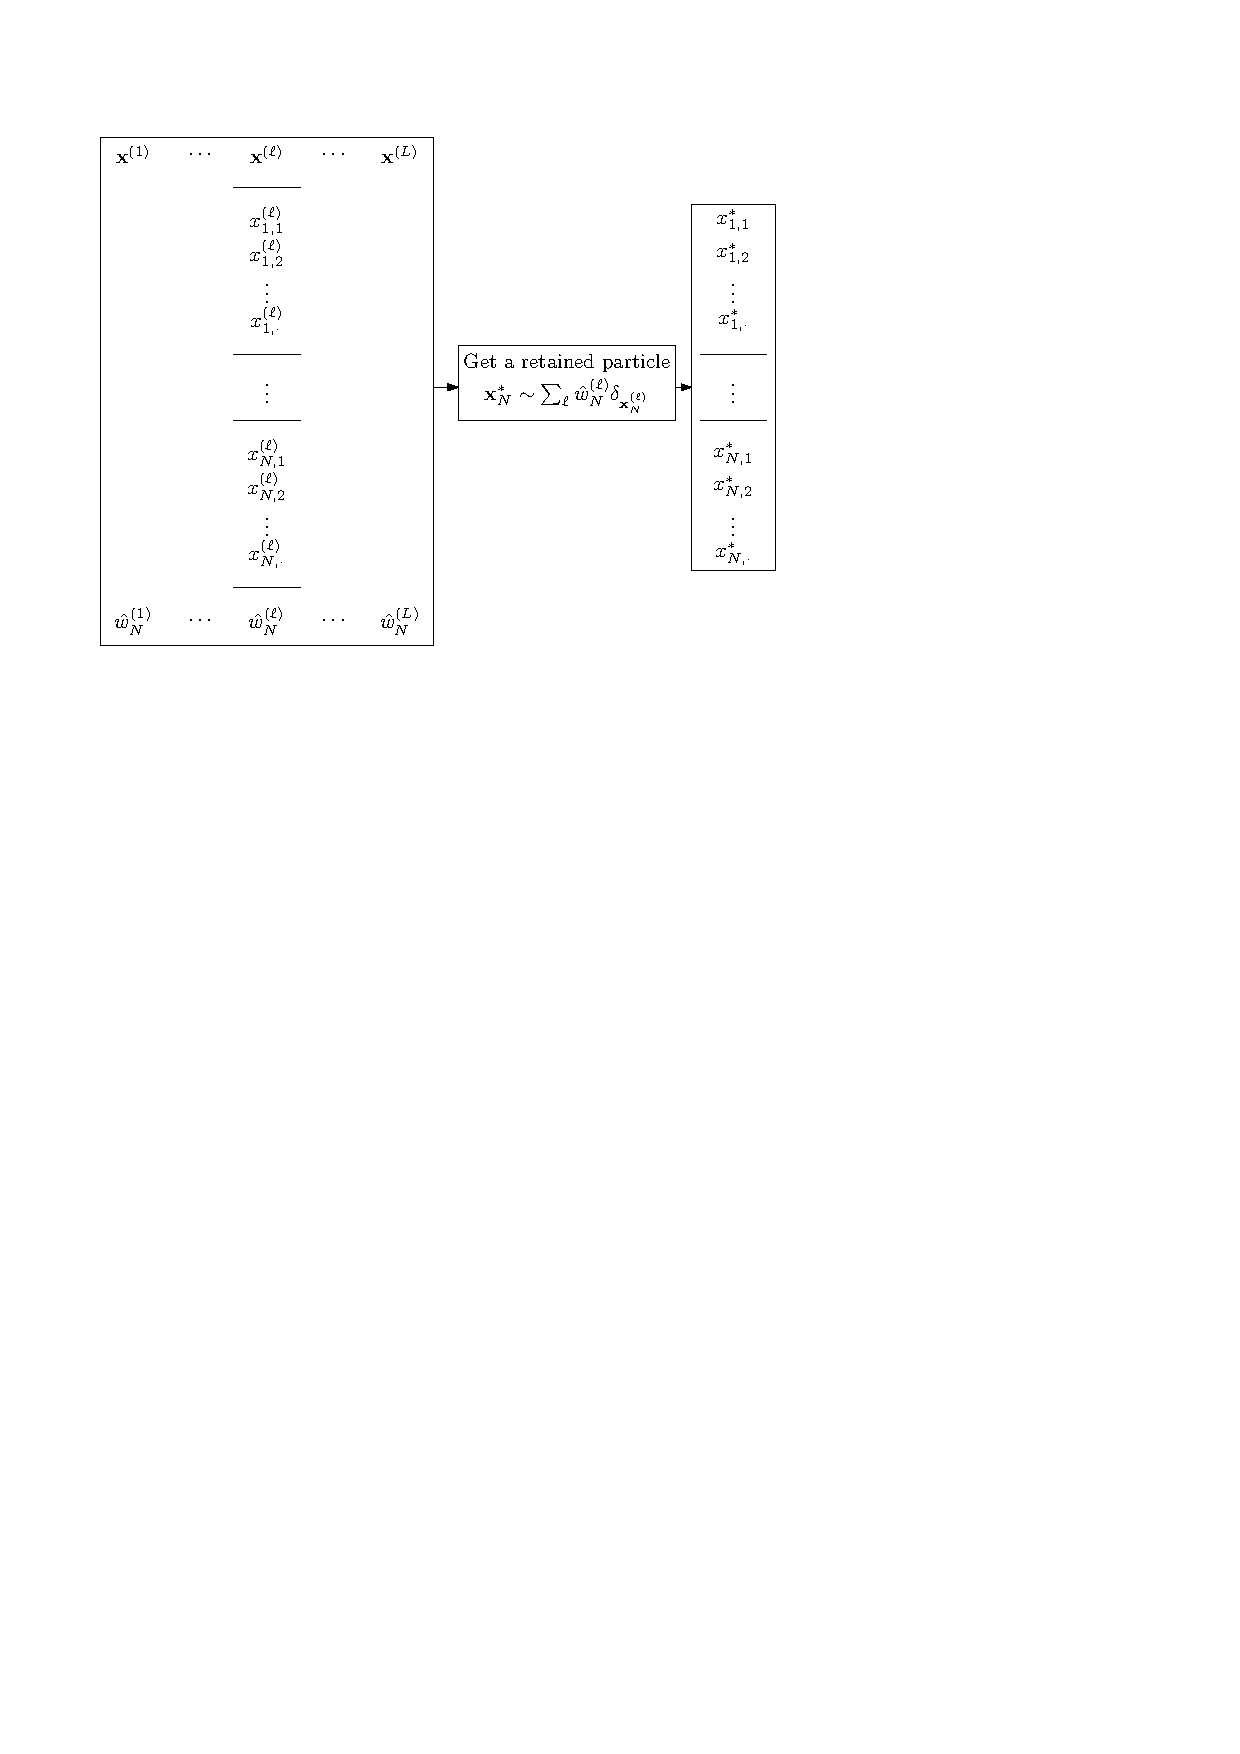
\includegraphics[scale=0.75]{pprog/how/figures/pgibbs/pgibbs1}
\caption{Initialisation of the Particle Gibbs sampler.}
\label{fig:pprog/how/figures/pgibbs1}
\end{figure}

\begin{figure}[!htb]
\centering
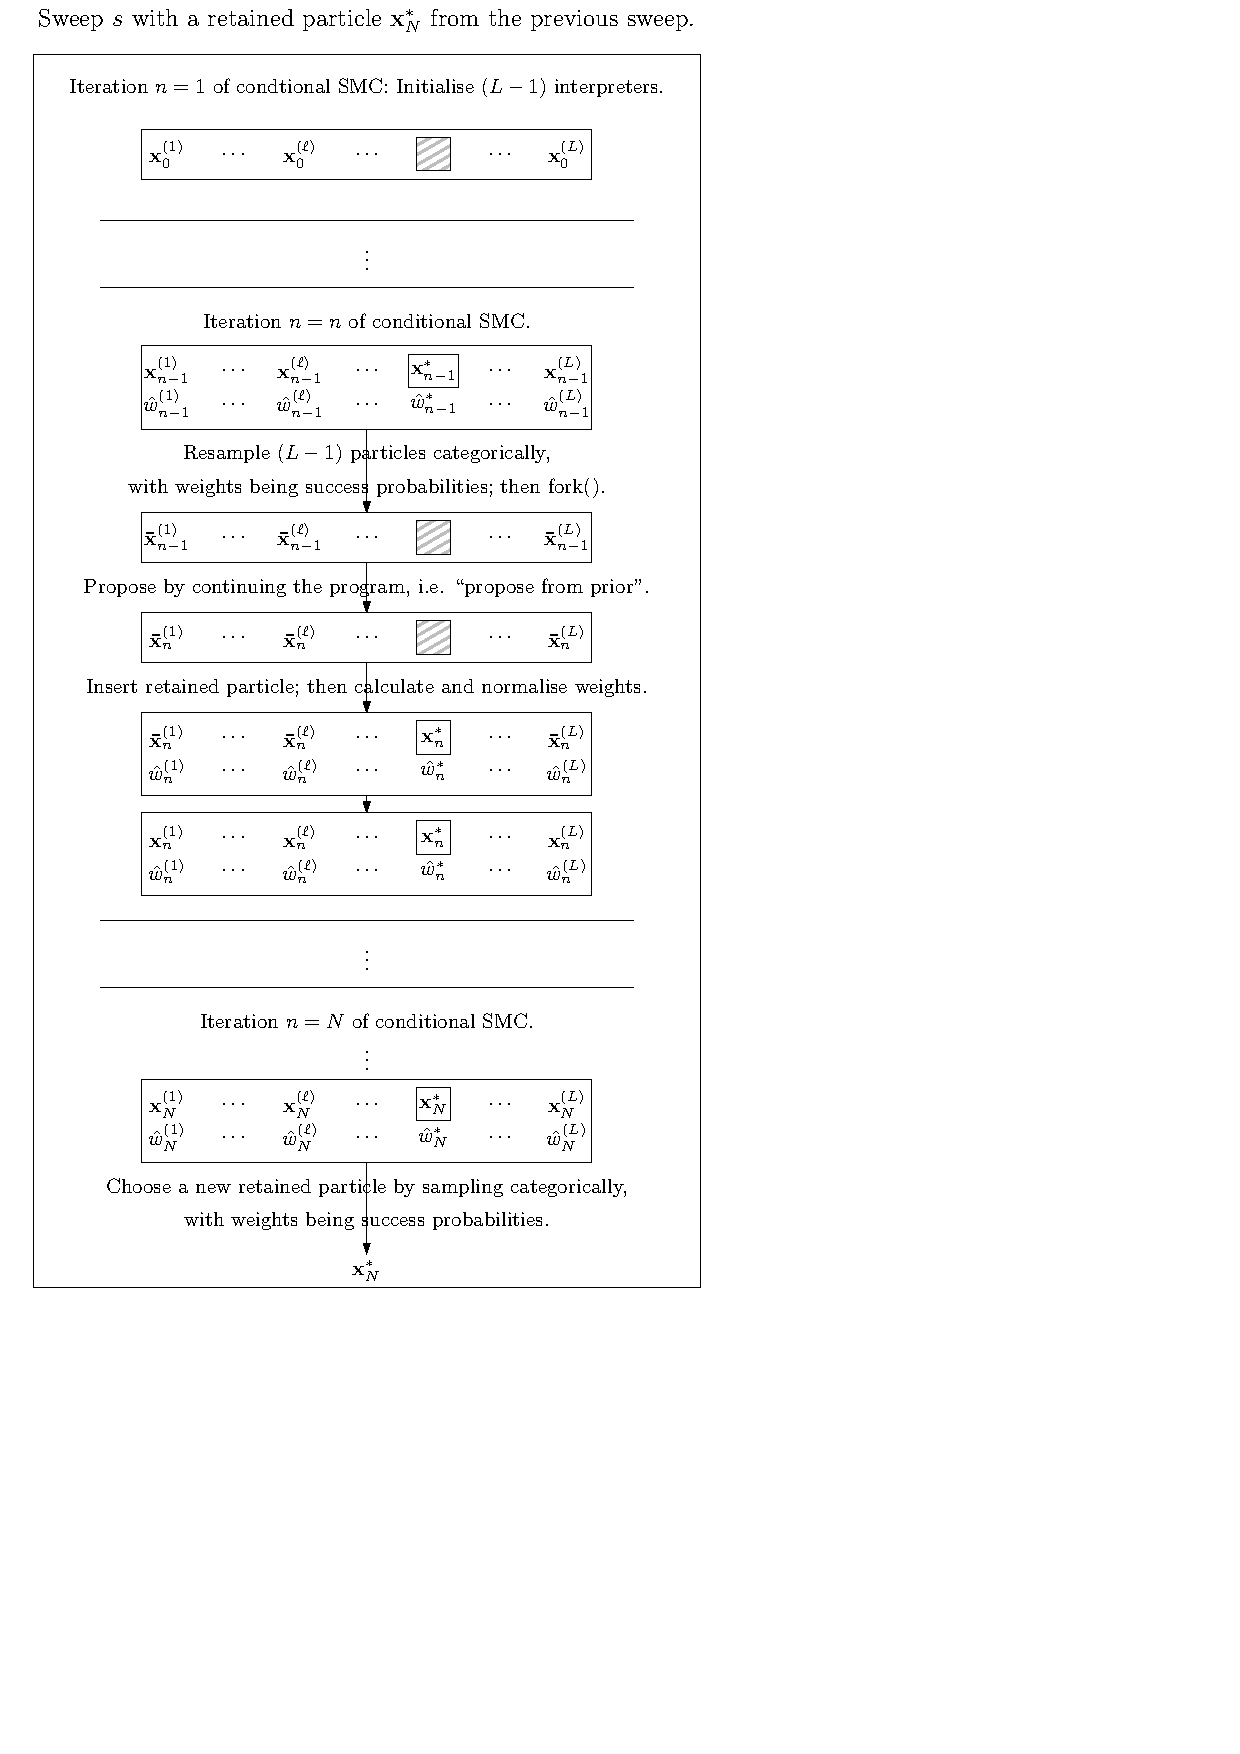
\includegraphics[scale=0.8]{pprog/how/figures/pgibbs/pgibbs2}
\caption{Sweep $s$ of the Particle Gibbs sampler.}
\label{fig:pprog/how/figures/pgibbs2}
\end{figure}